\begin{figure}[H]
    \centering
    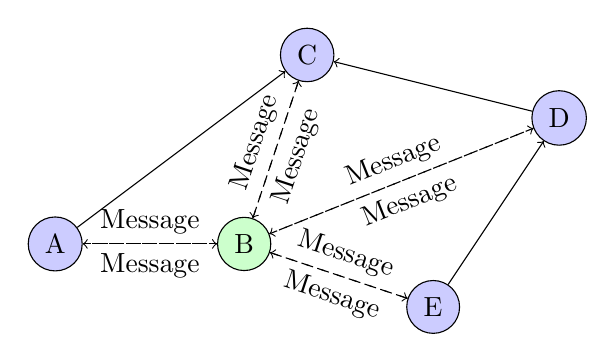
\begin{tikzpicture}[scale=0.8]
        \node[circle, draw, fill=blue!20] (A) at (0,0) {A};
        \node[circle, draw, fill=green!20] (B) at (3,0) {B};
        \node[circle, draw, fill=blue!20] (C) at (4,3) {C};
        \node[circle, draw, fill=blue!20] (D) at (8,2) {D};
        \node[circle, draw, fill=blue!20] (E) at (6,-1) {E};
        \draw[->] (A) -- (C);
        \draw[->] (D) -- (C);
        \draw[->] (E) -- (D);
        \draw[->, dashed] (A) -- (B) node[midway, above, sloped] {Message};
        \draw[->, dashed] (B) -- (A) node[midway, below, sloped] {Message};
        \draw[->, dashed] (C) -- (B) node[midway, above, sloped] {Message};
        \draw[->, dashed] (B) -- (C) node[midway, below, sloped] {Message};
        \draw[->, dashed] (B) -- (D) node[midway, above, sloped] {Message};
        \draw[->, dashed] (D) -- (B) node[midway, below, sloped] {Message};
        \draw[->, dashed] (B) -- (E) node[midway, below, sloped] {Message};
        \draw[->, dashed] (E) -- (B) node[midway, above, sloped] {Message};
    \end{tikzpicture}
    \caption{Message passing between node B and its neighbors in a GNN.}
    \label{fig:gnn}
\end{figure}